\subsection{Mathematik I}

Was ist das Gegenteil der Aussage \glqq Auf beiden Klassenfahrten haben alle
Schüler jeden Tag gebadet?\grqq\ Kann man eine Strecke der Länge 10 so in zwei
Stücke zerlegen, dass das aus ihnen gebildete Rechteck den Flächeninhalt 41
hat? Wie viele Brötchen muss man mindestens schmieren, damit mit 90\%-iger
Wahrscheinlichkeit alle satt werden, wenn man 12 Gäste eingeladen hat, von
denen jeder mit Wahrscheinlichkeit $\frac 1 4$ entweder 1,2 oder 3 Brötchen
essen möchte? Und was ist eigentlich $2^\pi$?

Solche und ähnliche Fragen möchte ich in den kommenden Semestern mit Ihnen
diskutieren -- dabei werden wir auf der Suche nach den entsprechenden
Antworten, was unsere mathematischen Kenntnisse betrifft, noch einmal ganz weit
zurück gehen und den Erkenntnisgewinn aus einer anderen Perspektive -- der
sogenannten \emph{axiomatischen} -- aufrollen. Hierbei werden Sie merken, dass
sich die Mathematik an der Universität in einem ganz anderen Gewand präsentiert
als in der Schule; es gibt mit Sicherheit viel Spannendes und Neues zu
entdecken und zu lernen! Vieles hiervon werden Sie später in der Schule in der
an der Universität dargebotenen Form nicht vermitteln (können) -- zum einen
sind die Inhalte mitunter zu anspruchsvoll für die Primar- und Sekundarstufe I
bzw. für die Sonderschule, zum anderen ist die Darstellung zu abstrakt -- aber
ich versichere Ihnen, dass das in diesem Studiengang zu erwerbende
mathematische Wissen unverzichtbares und wertvolles Hintergrundwissen für die
Ausübung Ihres Berufs darstellen wird! In Anbetracht der Tatsache, dass Sie
Lehrerinnen und Lehrer werden möchten, werde ich außerdem in besonderem Maße
versuchen, immer wieder den Schulbezug der verschiedenen Lehrinhalte
aufzuzeigen.

\begin{wrapfigure}{l}{35mm}
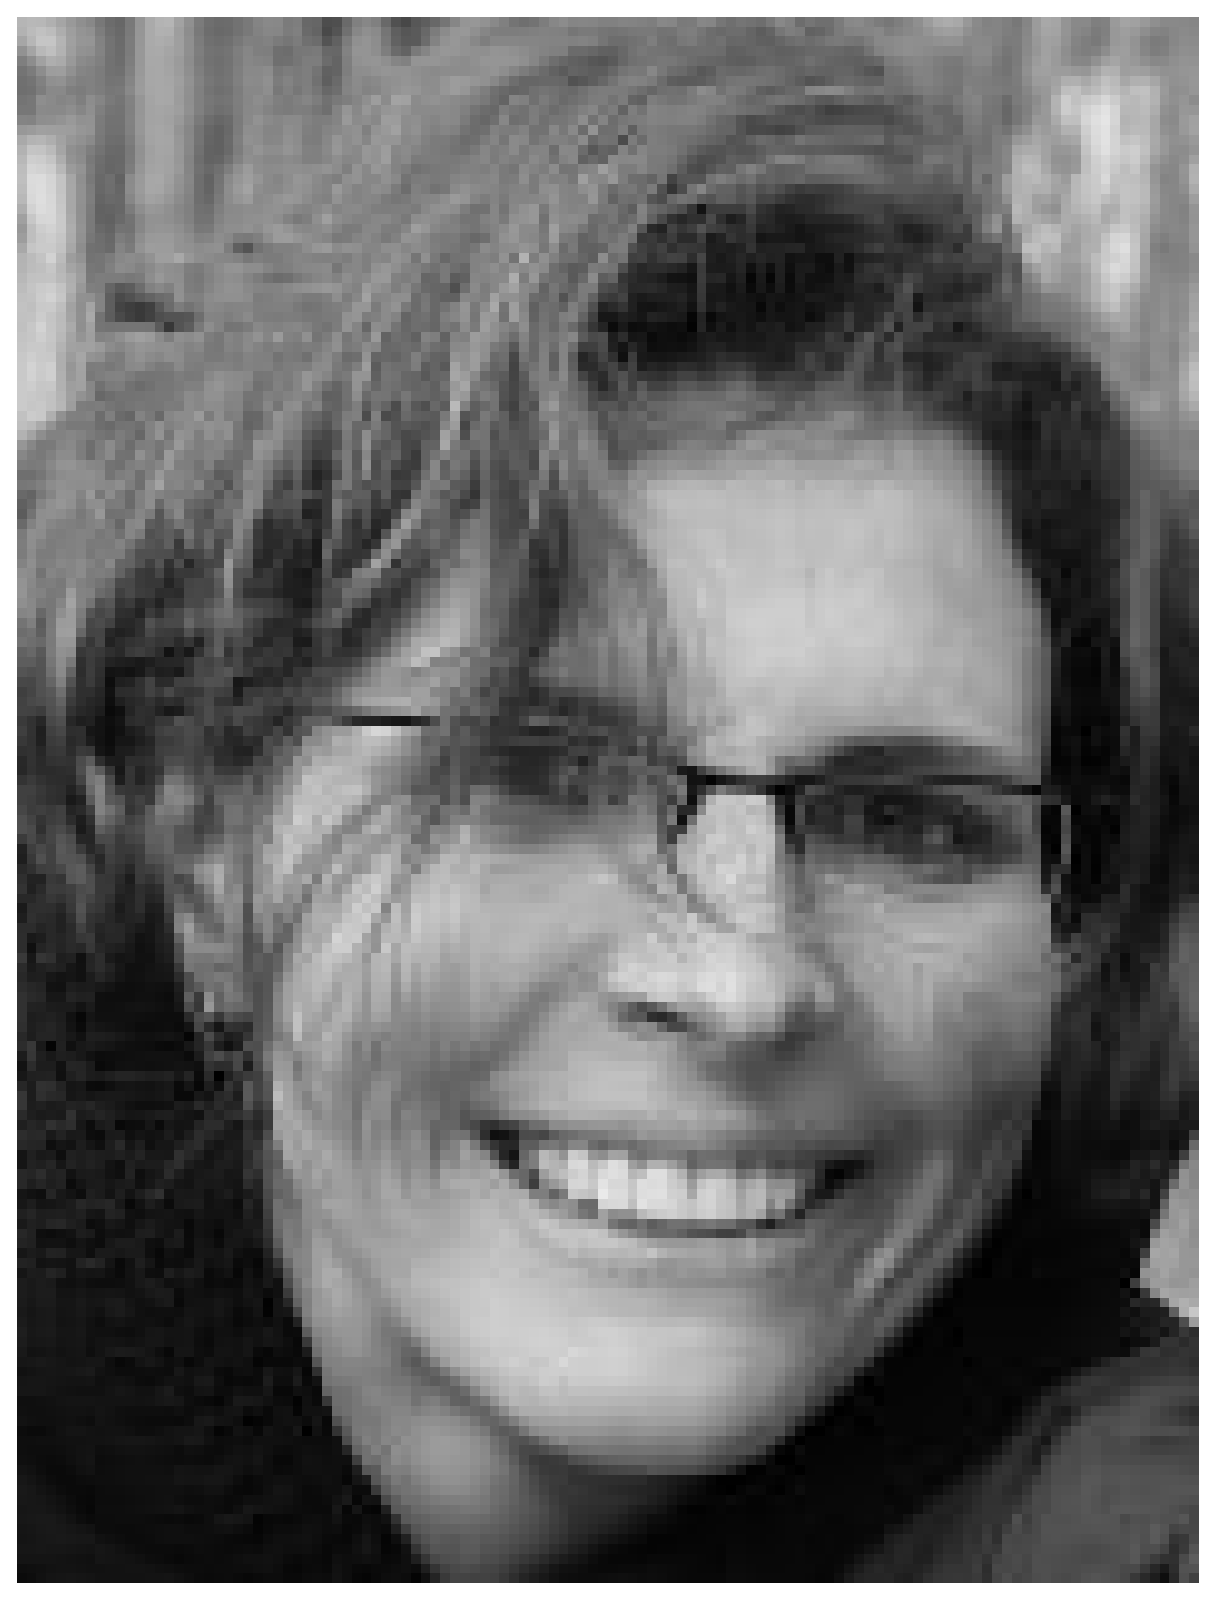
\includegraphics[scale=0.15]{images/koch}
\end{wrapfigure}

Mein Interesse für die Ausbildung angehender Lehrerinnen und Lehrer entspricht
meiner eigenen Biographie: Von 1991 bis 1996 habe ich nämlich in Göttingen
selbst Mathematik und Physik für das Lehramt an Gymnasien studiert. Die große
Freude, die mir das Mathematikstudium bereitet hat, führte dazu, dass ich im
Anschluss daran mit der Forschung an wahrscheinlichkeitstheoretischen
Fragestellungen begann. Im Rahmen verschiedener Anstellungen in Texas und
Göttingen habe ich neben meiner Forschungstätigkeit aber immer auch intensiv an
der Ausbildung junger Menschen in Mathematik mitgewirkt, insbesondere für
Lehramtsstudierende. Zum Sommersemester 2006 bin ich an die Universität Hamburg
gekommen, wo ich seitdem mit der Ausbildung der Studierenden des Lehramts für
die Primar- und Sekundarstufe I bzw. an Sonderschulen betraut bin.

Ich freue mich darauf, Sie in den kommenden Wochen näher kennen zu lernen und
mit Ihnen eine mehrsemestrige Reise durch die wunderbare Welt der Mathematik zu
machen. Bis dahin wünsche ich Ihnen eine gute Zeit während der
Orientierungswochen und einen erfolgreichen Start ins Studium!

\hfill Susanne Koch
